\documentclass[preview]{standalone}

%graphics
\usepackage{xcolor}
\usepackage{tikz}
\usetikzlibrary{shapes.geometric, shapes.multipart, arrows, calc, through}
\usepackage[caption=false,font=footnotesize]{subfig}

\colorlet{dot-color}{black!80}
\tikzset{
    pics/cell/.style = {
        code = {%
        \coordinate (-center) at (0,0);
        
        \fill +(-0.245,-0.245) coordinate(-sw) 
           -- +(-0.245, 0.245) coordinate(-nw)
           -- +( 0.245, 0.245) coordinate(-ne)
           -- +( 0.245,-0.245) coordinate(-se)
           -- cycle;
        \coordinate (-swo) at ($ (-center)!0.5!(-sw) $);
        \coordinate (-nwo) at ($ (-center)!0.5!(-nw) $);
        \coordinate (-neo) at ($ (-center)!0.5!(-ne) $);
        \coordinate (-seo) at ($ (-center)!0.5!(-se) $);
        
        \coordinate (-south) at ($ (-sw)!.5!(-se) $);
        \coordinate (-north) at ($ (-nw)!.5!(-ne) $);
        \coordinate (-west)  at ($ (-sw)!.5!(-nw) $);
        \coordinate (-east)  at ($ (-se)!.5!(-ne) $);
        
        \fill[white] (-swo) let \p1=($ (-center)!.5!(-swo) $) in circle ({veclen(\x1,\y1)});
        \fill[white] (-nwo) let \p1=($ (-center)!.5!(-nwo) $) in circle ({veclen(\x1,\y1)});
        \fill[white] (-neo) let \p1=($ (-center)!.5!(-neo) $) in circle ({veclen(\x1,\y1)});
        \fill[white] (-seo) let \p1=($ (-center)!.5!(-seo) $) in circle ({veclen(\x1,\y1)});
        
        \ifnum#1=1\relax
            \fill[dot-color] (-swo) let \p1=($ (-center)!.32!(-swo) $) in circle ({veclen(\x1,\y1)});
            \fill[dot-color] (-neo) let \p1=($ (-center)!.32!(-neo) $) in circle ({veclen(\x1,\y1)});
        \else
            \ifnum#1=-1\relax
                \fill[dot-color] (-nwo) let \p1=($ (-center)!.32!(-nwo) $) in circle ({veclen(\x1,\y1)});
                \fill[dot-color] (-seo) let \p1=($ (-center)!.32!(-seo) $) in circle ({veclen(\x1,\y1)});
            \else
                \fill[dot-color] (-swo) let \p1=($ (-center)!.22!(-swo) $) in circle ({veclen(\x1,\y1)});
                \fill[dot-color] (-nwo) let \p1=($ (-center)!.22!(-nwo) $) in circle ({veclen(\x1,\y1)});
                \fill[dot-color] (-neo) let \p1=($ (-center)!.22!(-neo) $) in circle ({veclen(\x1,\y1)});
                \fill[dot-color] (-seo) let \p1=($ (-center)!.22!(-seo) $) in circle ({veclen(\x1,\y1)});
            \fi
        \fi
        }
    },
    pics/cell/.default={0}
}
% \definecolor{clock0}{HTML}{86E291}
% \definecolor{clock1}{HTML}{FFA5FA}
% \definecolor{clock2}{HTML}{00C8BC}
% \definecolor{clock3}{HTML}{F2F2F2}
% \definecolor{input}{HTML}{008DC8}
% \definecolor{output}{HTML}{E28686}
% \definecolor{fixed}{HTML}{000000}

\definecolor{clock0}{RGB}{89,89,91}
\definecolor{clock1}{RGB}{129,130,132}
\definecolor{clock2}{RGB}{210,210,212}
\definecolor{clock3}{RGB}{168,169,173}
\definecolor{input}{RGB}{230,230,230}
\definecolor{output}{RGB}{40,40,40}
\definecolor{fixed}{HTML}{000000}


\begin{document}

\begin{figure}[!t]
\centering
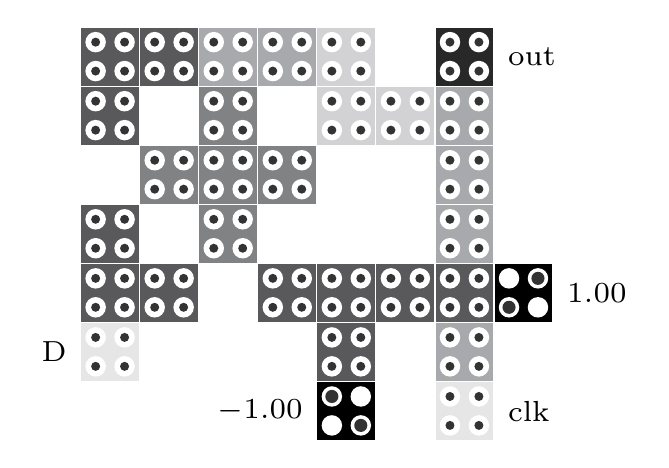
\begin{tikzpicture}[scale=1.5,transform shape]
\pic(i1)[input]  at (0,0.5) {cell};
\node [left] at (i1-west) {\scriptsize D};
\pic[clock0] at (0,1) {cell};
\pic[clock0] at (0,1.5) {cell};
\pic[clock0] at (0,2.5) {cell};
\pic[clock0] at (0,3) {cell};

\pic[clock0] at (0.5,1) {cell};
\pic[clock1] at (0.5,2) {cell};
\pic[clock0] at (0.5,3) {cell};

\pic[clock1] at (1,1.5) {cell};
\pic[clock1] at (1,2) {cell};
\pic[clock1] at (1,2.5) {cell};
\pic[clock3] at (1,3) {cell};

\pic[clock0] at (1.5,1) {cell};
\pic[clock1] at (1.5,2) {cell};
\pic[clock3] at (1.5,3) {cell};

\pic(f1)[fixed] at (2,0) {cell=-1};
\node[left] at (f1-west) {\scriptsize $-1.00$};
\pic[clock0] at (2,0.5) {cell};
\pic[clock0] at (2,1) {cell};
\pic[clock2] at (2,2.5) {cell};
\pic[clock2] at (2,3) {cell};

\pic[clock0] at (2.5,1) {cell};
\pic[clock2] at (2.5,2.5) {cell};

\pic(i2)[input] at (3,0) {cell};
\node [right] at (i2-east) {\scriptsize clk};
\pic[clock3] at (3,0.5) {cell};
\pic[clock0] at (3,1) {cell};
\pic[clock3] at (3,1.5) {cell};
\pic[clock3] at (3,2) {cell};
\pic[clock3] at (3,2.5) {cell};
\pic(o1)[output] at (3,3) {cell};
\node [right] at (o1-east) {\scriptsize out};

\pic(f2)[fixed] at (3.5,1) {cell=1};
\node [right] at (f2-east) {\scriptsize $1.00$};
\end{tikzpicture}
\end{figure}

\end{document}
